\documentclass[10pt]{article}
\usepackage[letterpaper,margin=0.68in,headheight=14pt]{geometry}
\usepackage[T1]{fontenc}
\usepackage{lmodern}
\usepackage{microtype}
\usepackage{graphicx}
\usepackage{booktabs}
\usepackage{tabularx}
\usepackage{array}
\usepackage[table]{xcolor}
\usepackage{enumitem}
\usepackage{caption}
\usepackage{float}
\usepackage{titlesec}
\usepackage{fancyhdr}
\usepackage[hidelinks]{hyperref}

\definecolor{navy}{HTML}{1F3A5F}
\definecolor{blue}{HTML}{245D91}
\definecolor{teal}{HTML}{0F766E}
\definecolor{lightblue}{HTML}{E8EEF5}
\definecolor{lightgrey}{HTML}{F2F4F7}
\definecolor{bestgreen}{HTML}{E7F4EC}

\pagestyle{fancy}
\fancyhf{}
\lhead{\footnotesize LOCO Anomaly Inspector | Data Analytics Lab Final Report}
\rfoot{\footnotesize Page \thepage}
\renewcommand{\headrulewidth}{0.3pt}
\renewcommand{\footrulewidth}{0pt}

\titleformat{\section}{\large\bfseries\color{blue}}{\thesection.}{0.45em}{}
\titleformat{\subsection}{\normalsize\bfseries\color{navy}}{\thesubsection}{0.45em}{}
\titlespacing*{\section}{0pt}{5pt}{3pt}
\titlespacing*{\subsection}{0pt}{4pt}{2pt}
\setlist[itemize]{leftmargin=1.25em,itemsep=1pt,topsep=2pt}
\setlist[enumerate]{leftmargin=1.35em,itemsep=1pt,topsep=2pt}
\captionsetup{font=footnotesize,labelfont=bf,skip=2pt}
\setlength{\parindent}{0pt}
\setlength{\parskip}{3pt}
\renewcommand{\arraystretch}{1.08}

\begin{document}
\fontsize{9.4}{10.8}\selectfont

% Add student name, ID, and institution below if your faculty requires them.
\begin{center}
{\LARGE\bfseries\color{navy} LOCO Anomaly Inspector}\\[2pt]
{\large\itshape Logical and Structural Anomaly Detection on MVTec LOCO AD}\\[3pt]
{\small\bfseries\color{teal} Data Analytics Lab | Final Project Report | June 2026}
\end{center}
\vspace{-2pt}
\hrule height 0.8pt
\vspace{5pt}

\colorbox{lightgrey}{%
\parbox{\dimexpr\linewidth-2\fboxsep\relax}{%
\textbf{Abstract.} This project detects industrial product defects using only normal
training images. Frozen DINOv2-small features support three anomaly detectors, while a
lightweight global proxy provides an additional baseline. The system compares seven
scoring configurations and presents the results in Power BI and an offline HTML
dashboard. Mean fusion achieved 0.761 overall AUROC, with stronger performance on
structural anomalies than logical anomalies.}}

\section{Introduction}
Industrial inspection systems must find uncommon defects before products reach
customers. In practice, defective examples are limited and expensive to label.
Anomaly detection addresses this problem by learning the appearance of normal products
and assigning a higher score to unusual test images.

\begin{itemize}
\item \textbf{Structural anomalies:} local visual defects such as damage,
contamination, or deformation.
\item \textbf{Logical anomalies:} missing, extra, misplaced, or incorrectly counted
parts that may still look normal.
\end{itemize}

The study uses all five MVTec LOCO AD categories: breakfast box, juice bottle,
pushpins, screw bag, and splicing connectors. The audited data contains 3,651 images
across normal training, normal validation, and held-out test splits.

\section{Objective of the Product}
The objective is to build a clear anomaly-detection product that can:
\begin{itemize}
\item \textbf{Detect} normal and abnormal images without training on defects.
\item \textbf{Compare} logical, structural, overall AUROC, and F1.
\item \textbf{Explain} scores, thresholds, ground truth, and model heatmaps separately.
\item \textbf{Support review} by placing useful EDA and model evidence in one dashboard.
\end{itemize}

\begin{center}
\rowcolors{1}{lightblue}{lightblue}
\begin{tabular}{>{\centering\arraybackslash}p{0.22\linewidth}
                >{\centering\arraybackslash}p{0.22\linewidth}
                >{\centering\arraybackslash}p{0.22\linewidth}
                >{\centering\arraybackslash}p{0.22\linewidth}}
\textbf{\large 0.761} & \textbf{\large 0.731} & \textbf{\large 0.804} & \textbf{\large 5}\\
\footnotesize Overall AUROC & \footnotesize Logical AUROC &
\footnotesize Structural AUROC & \footnotesize Product categories
\end{tabular}
\end{center}

\newpage
\section{Product Features}
The product is available as a Power BI dashboard and as a self-contained HTML
dashboard. Both versions focus on evidence needed to understand the model.
\begin{itemize}
\item \textbf{Overview and leaderboard:} show the best method and all seven scoring configurations.
\item \textbf{Relevant EDA:} show split counts, sample images, mask overlays, and category patterns.
\item \textbf{Explainability and drill-down:} show per-image decisions, category results, thresholds, and heatmaps.
\end{itemize}

\begin{figure}[H]
\centering
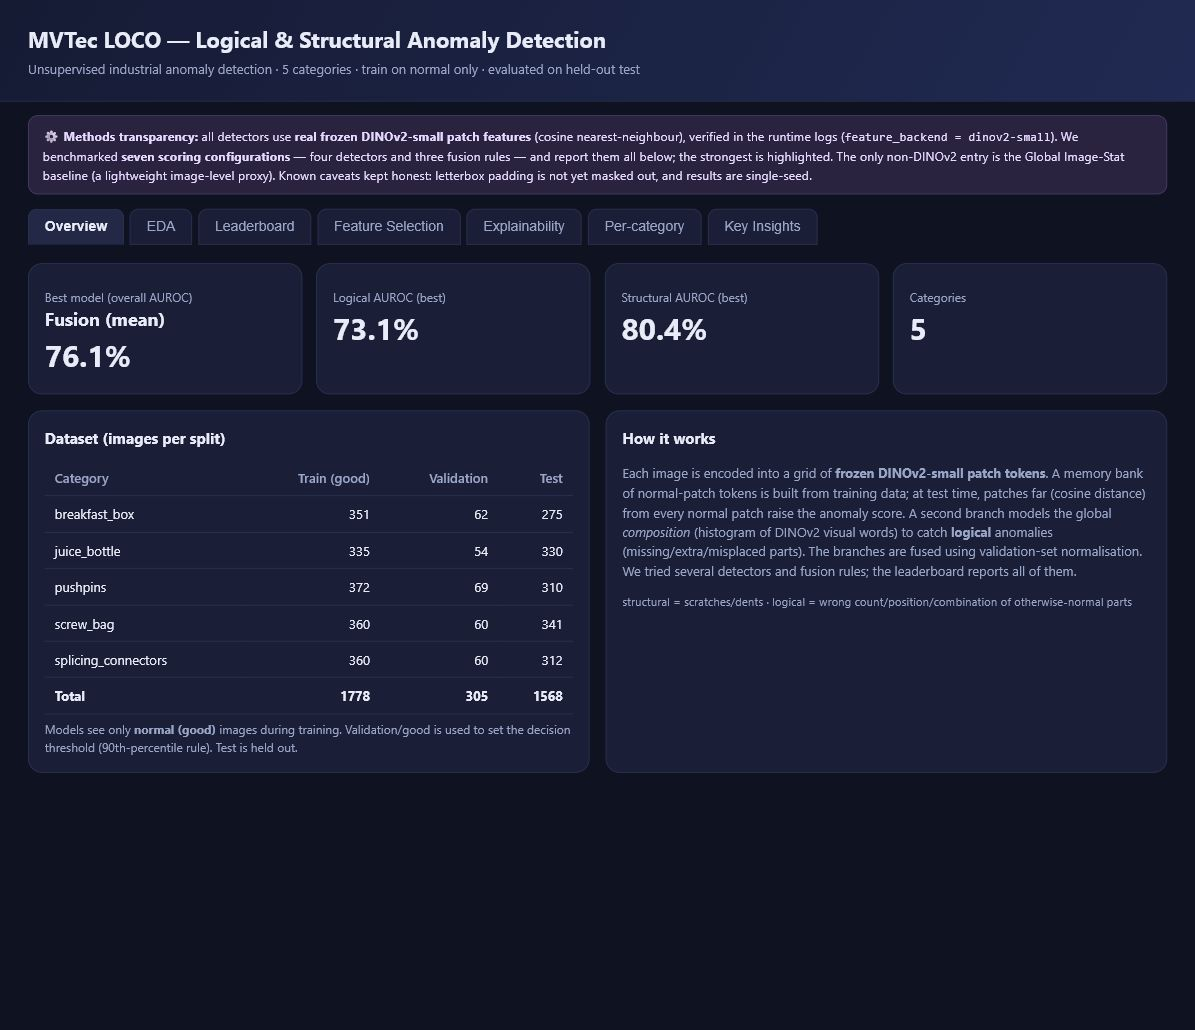
\includegraphics[width=0.86\linewidth]{figures/dashboard_overview.png}
\caption{Dashboard overview showing the headline metrics, dataset split, and method transparency statement.}
\end{figure}

\section{User Guidelines}
\begin{enumerate}
\item \textbf{Open the dashboard.} Use the Power BI file or open
\texttt{09\_dashboard/dashboard.html}.
\item \textbf{Read the overview.} Check overall, logical, and structural AUROC.
\item \textbf{Use a detailed tab.} Select the leaderboard, explainability, or per-category view.
\item \textbf{Interpret a decision.} A score at or above the saved validation threshold is flagged as anomalous.
\end{enumerate}

\newpage
\section{Implementation and Methodology}
\begin{figure}[H]
\centering
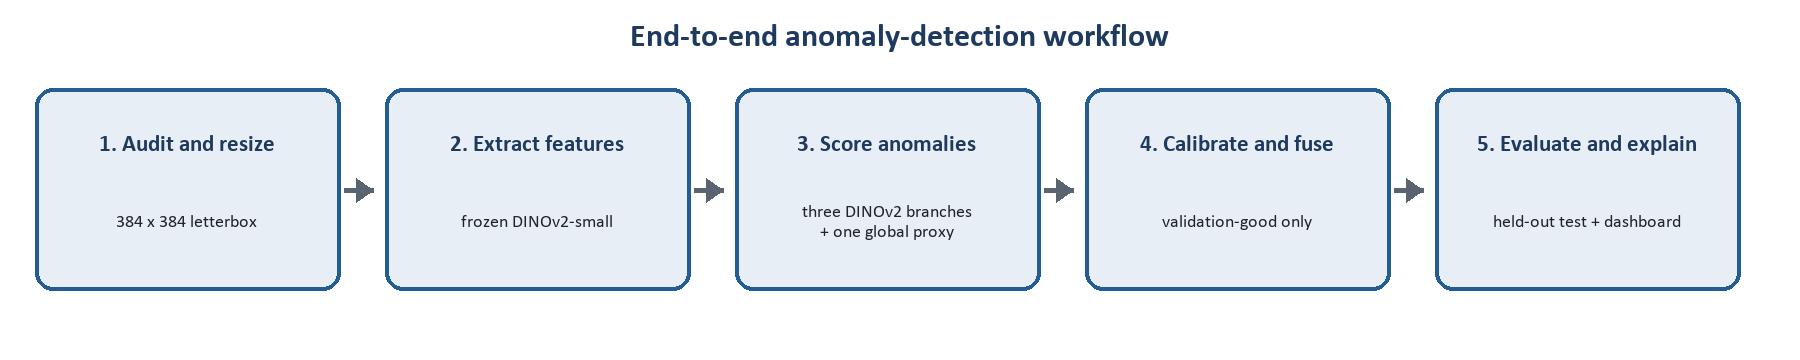
\includegraphics[width=\linewidth]{figures/pipeline.png}
\caption{End-to-end workflow from data preparation to dashboard reporting.}
\end{figure}

\subsection{Data Preparation}
Images are placed on a 384 $\times$ 384 canvas using aspect-ratio-preserving
letterboxing. Product images use bilinear interpolation. Ground-truth masks use
nearest-neighbour interpolation and remain binary. Only normal images are used to fit
the anomaly detectors.

\subsection{Model Methods}
\begin{table}[H]
\centering
\footnotesize
\begin{tabularx}{\linewidth}{>{\bfseries}p{0.23\linewidth}X p{0.20\linewidth}}
\toprule
Detector branch & Purpose & Feature source\\
\midrule
Patch Memory & Find local patches unlike the normal memory bank. & DINOv2-small\\
Region-Aware Memory & Compare appearance while keeping rough image position. & DINOv2-small\\
Composition Histogram & Measure changes in the global mix of visual words. & DINOv2-small\\
Global Image-Stat proxy & Provide a fast whole-image difference score. & Non-DINOv2 proxy\\
\bottomrule
\end{tabularx}
\caption{Detector branches used in the reported comparison.}
\end{table}

The three DINOv2 branches use real frozen DINOv2-small patch features. The Global
Image-Stat detector is a lightweight non-DINOv2 proxy. Mean, maximum, and rank-average
fusion combine the branch scores. This report does not claim an official EfficientAD
or PatchCore implementation.

\subsection{Evaluation Protocol}
\begin{itemize}
\item \textbf{Training:} fit normal memories using train/good images.
\item \textbf{Calibration:} use validation/good scores for normalization and the 90th-percentile threshold.
\item \textbf{Testing:} use the held-out test split only for final evaluation.
\item \textbf{Metrics:} report image-level AUROC and F1; AUROC is the main comparison metric.
\end{itemize}

\newpage
\section{Results and Feature Selection}
\begin{table}[H]
\centering
\scriptsize
\begin{tabularx}{\linewidth}{Xrrrr}
\toprule
Method & Logical & Structural & Overall & F1\\
\midrule
\rowcolor{bestgreen} Fusion (mean) & 0.731 & 0.804 & 0.761 & 0.626 \\
Region-Aware Memory & 0.730 & 0.784 & 0.750 & 0.626 \\
Patch Memory & 0.697 & 0.765 & 0.724 & 0.612 \\
Fusion (rank average) & 0.727 & 0.720 & 0.720 & 0.573 \\
Fusion (max) & 0.692 & 0.741 & 0.714 & 0.551 \\
Global Image-Stat proxy & 0.634 & 0.683 & 0.655 & 0.474 \\
Composition Histogram & 0.644 & 0.498 & 0.576 & 0.396 \\
\bottomrule
\end{tabularx}
\caption{Corrected image-level results. AUROC is threshold-free; F1 uses a validation-good operating threshold.}
\end{table}

\begin{figure}[H]
\centering
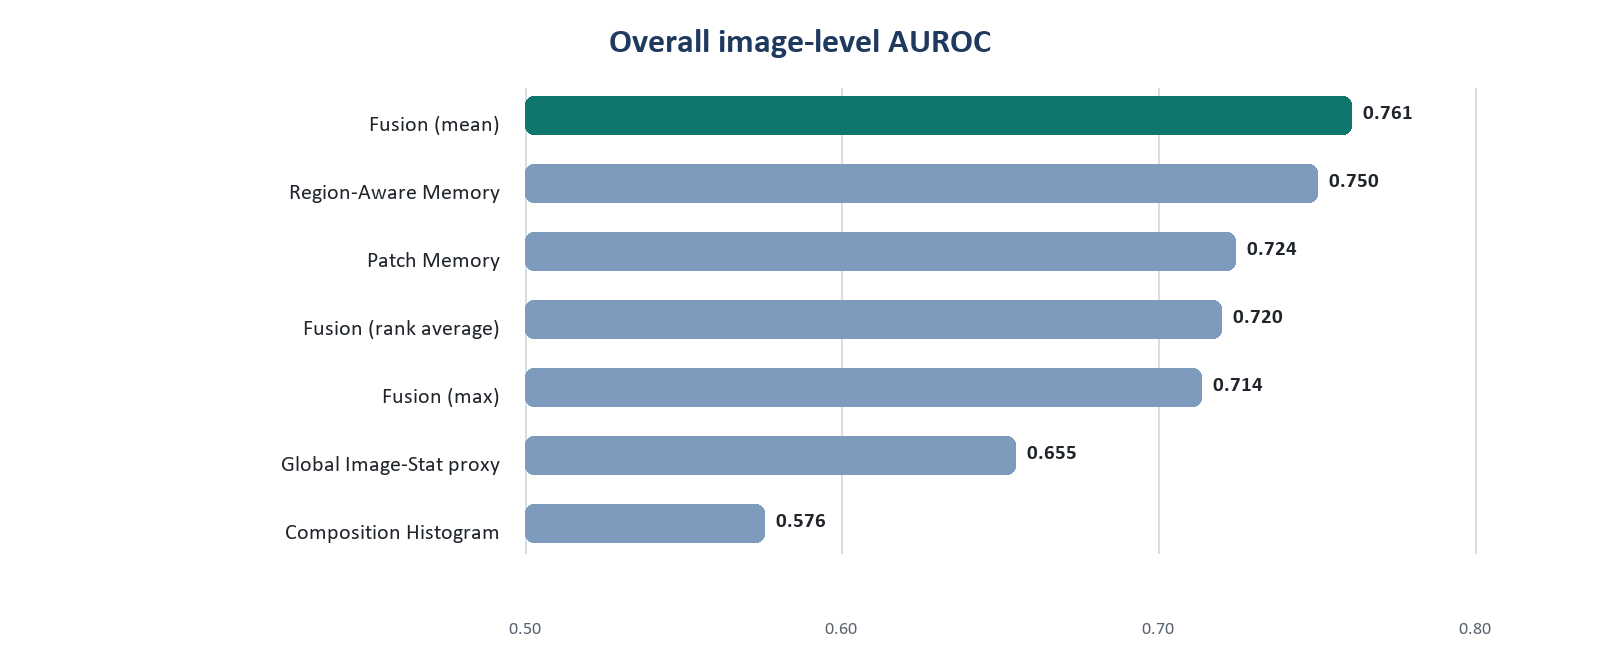
\includegraphics[width=0.95\linewidth]{figures/results_chart.png}
\caption{Corrected overall AUROC for all reported methods and fusion rules.}
\end{figure}

\begin{itemize}
\item \textbf{Best pre-specified result:} mean fusion reached 0.761 overall AUROC.
\item \textbf{Best single detector:} Region-Aware Memory reached 0.750 overall AUROC.
\item \textbf{Main pattern:} structural AUROC (0.804) was higher than logical AUROC (0.731).
\end{itemize}

\colorbox{bestgreen}{%
\parbox{\dimexpr\linewidth-2\fboxsep\relax}{%
\textbf{Feature-selection analysis.} Removing a duplicate Patch Memory entry and the
weak Composition Histogram branch produced a three-branch score of 0.764 overall AUROC
and 0.826 structural AUROC. This analysis used held-out test labels, so it is reported
as a later diagnostic result. Mean fusion remains the headline result.}}

\newpage
\section{Explainability and Limitations}
\begin{figure}[H]
\centering
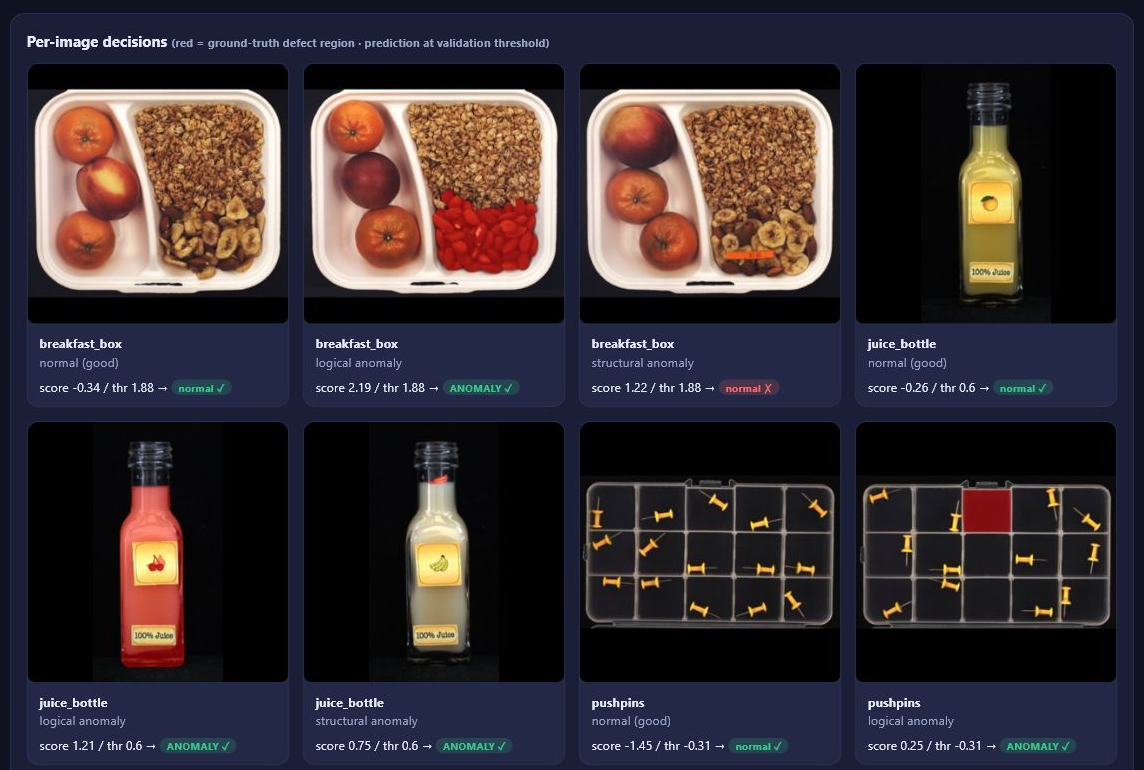
\includegraphics[width=0.88\linewidth]{figures/explainability_decisions.png}
\caption{Per-image decisions with anomaly score, validation threshold, predicted class, and ground-truth defect region.}
\end{figure}

The red region is the dataset annotation, while the score and prediction are model
outputs. Keeping them separate prevents the ground truth from being mistaken for a
generated explanation.

\begin{itemize}
\item \textbf{Single run:} the headline experiment has not been repeated across several random seeds.
\item \textbf{Padding:} letterbox padding is not fully removed from patch modelling and scoring.
\item \textbf{Logical reasoning:} nearest-neighbour features do not explicitly count parts or model long-range relations.
\item \textbf{Localization:} the final comparison does not yet include complete pixel AUROC and AUPRO results.
\end{itemize}

\section{Conclusion}
The LOCO Anomaly Inspector meets the project requirements by combining unsupervised
anomaly detection, method comparison, useful EDA, and an interactive dashboard. Mean
fusion achieved 0.761 overall AUROC, and the Region-Aware branch was the strongest
single detector. The results also show that logical anomalies remain harder than
visible structural defects.

\section*{References}
\footnotesize
[1] Bergmann et al., MVTec LOCO AD and GCAD, \textit{International Journal of Computer Vision}, 2022.\\
[2] Oquab et al., DINOv2: Learning Robust Visual Features without Supervision, \textit{TMLR}, 2024.\\
[3] MVTec LOCO AD dataset documentation and project experiment outputs.

\end{document}
